% -----------------------------------------------
% Template for ISMIR Papers
% 2023 version, based on previous ISMIR templates

% Requirements :
% * 6+n page length maximum
% * 10MB maximum file size
% * Copyright note must appear in the bottom left corner of first page
% * Clearer statement about citing own work in anonymized submission
% (see conference website for additional details)
% -----------------------------------------------

\documentclass{article}
\usepackage{lineno}
\linenumbers
\usepackage[T1]{fontenc} % add special characters (e.g., umlaute)
\usepackage[utf8]{inputenc} % set utf-8 as default input encoding
\usepackage{ismir,amsmath,cite,url}
\usepackage{graphicx}
\usepackage{color}
\usepackage{pdfpages} % for including PDF files
\usepackage{multirow}
\usepackage{booktabs}
\usepackage{tabularx}
\usepackage{adjustbox}

% Title. Please use IEEE-compliant title case when specifying the title here,
% as it has implications for the copyright notice
% ------
\title{Towards a systematic exploration of motif development in Arab-Andalusian Music}

% Note: Please do NOT use \thanks or a \footnote in any of the author markup

% Single address
% To use with only one author or several with the same address
% ---------------
%\oneauthor
% {Names should be omitted for double-blind reviewing}
% {Affiliations should be omitted for double-blind reviewing}

% Two addresses
% --------------
%\twoauthors
%  {First author} {School \\ Department}
%  {Second author} {Company \\ Address}

% Three addresses
% --------------\input{ISMIR2021_paper.tex}

\threeauthors
  {Oriol Colomé i Font} {UPF \\ {\tt oriol.colome01@estudiant.upf.edu}}
  {} {}
  {Satyajeet Prabhu} {UPF \\ {\tt satyajeet.prabhu01@estudiant.upf.edu}}

% Four or more addresses
% OR alternative format for a large number of co-authors
% ------------
%\multauthor
%{First author$^1$ \hspace{1cm} Second author$^1$ \hspace{1cm} Third author$^2$} { \bfseries{Fourth author$^3$ \hspace{1cm} Fifth author$^2$ \hspace{1cm} Sixth author$^1$}\\
%  $^1$ Department of Computer Science, University, Country\\
%$^2$ International Laboratories, City, Country\\
%$^3$  Company, Address\\
%{\tt\small CorrespondenceAuthor@ismir.edu, PossibleOtherAuthor@ismir.edu}
%}

% For the author list in the Creative Common license, please enter author names. 
% Please abbreviate authors' first names and add 'and' between the second to last and last authors.
\def\authorname{O. Colome, and S. Prabhu}

% Optional: To use hyperref, uncomment the following.
%\usepackage[bookmarks=false,pdfauthor={\authorname},pdfsubject={\papersubject},hidelinks]{hyperref}
% Mind the bookmarks=false option; bookmarks are incompatible with ismir.sty.

\sloppy % please retain sloppy command for improved formatting

\begin{document}

%
\maketitle
%
\begin{abstract}

This paper investigates motif development in Arab-Andalusian Music in the \textit{al-Āla} tradition by studying repetition as a development technique to assess the centonization theory proposed by Amin Chachoo. We compare the significance, distribution, and repetition of critical motifs within a selected \textit{ṭab‘ (Iraq-al-ayam)} across multiple performances and across sections of a single performance. The key motifs (\textit{centos}) in the \textit{ṭab‘} used in this study are taken to be the intersection between those suggested by Chachoo and the significant motifs identified by Nuttall et al. through computational analysis in their study. Our analysis reveals patterns of cento repetition within delimited distinct musical structures. These repetitions appear purposeful, suggesting intentional compositional or improvisational decisions. Our findings support the idea that cento repetition in Arab-Andalusian music is systematic rather than arbitrary, indicating a potential structural and aesthetic significance of motif development within the tradition.

\end{abstract}
%
\section{Introduction}\label{sec:introduction}
Computational musicology has introduced innovative methods for analyzing music collections, allowing researchers to explore the many dimensions of music and its cultural significance in greater depth. \cite{Tzanetakis2007}\cite{Gomez&Herrera2013}

With the advent of digital recordings and software tools, we can systematically analyze large datasets and music performances in unprecedented ways. Although such approaches can complement traditional musicology, it is essential to recognize the subjective, cultural and inherently human nature of the music itself.\cite{towards_the_compleat_musicologist?}\cite{Jorna2011}

\subsection{Characteristics of Arab-Andalusian Music}\label{sec:characteristics}
\subsubsection{History and basic theory}\label{sec:history}
Arab-Andalusian music (AAM) is a rich musical tradition that emerged from the cultural fusion between the Muslim world and the Iberian Peninsula during the Al-Andalus period (8th to 15th centuries).

The central musical form in Arab-Andalusian music is the "\textbf{\textit{nawba}}". These suites serve as sonic journeys, encompassing instrumental and vocal compositions. Each nawba unfolds in a prescribed order dictated by the "\textbf{\textit{mīzān}}" (rhythmic mode). Traditionally, a nawba is unified by a primary "\textbf{\textit{ṭab‘}}" (melodic mode). Each ṭab‘, characterized by a specific diatonic scale and characteristic melodic motifs, is used to convey a certain emotional or spiritual content.\cite{opencorpus}

\subsubsection{Centonization Model}

Centonization (from Latin "\textit{cento}" meaning "patchwork") is a theory concerning the composition of melodies, or pieces, based on pre-defined melodic identities and formulas in music \cite{10.1093/mq/LX.3.333}\cite{10.2307/830914}. 

It is an old and widely used technique \cite{ferretti1977estetica} and similar concepts can be found in other musical traditions such as in Gregorian chant, the raga framework in Indian art music, or the pathet in Indonesian gamelan music.

\subsection{Motivation}\label{sec:motivation}

 With the aid of computation, this exploratory study seeks to observe macro patterns, if any, of centos development in AAM to deepen our understanding of the musical tradition. Specifically, we study the distribution, relative importance, and repetition of centos within a single ṭab‘ using musical transcriptions. Building upon existing computational analyses, we aim to contribute to the centonization theory in AAM proposed by Amin Chachoo \cite{Chaachoo2011} and also to gain a deeper musicological understanding of the tradition.

\section{Dataset}\label{sec:dataset}

CompMusic project \cite{compmusic} is the largest source of symbolic scores in the Arab-Andalusian tradition. It consists of 158 manual transcriptions of audio recordings of performances by three different orchestras done by Amin Chachoo. The scores are stored in the MusicXML\footnote{https://www.musicxml.com/} format and consist of a monophonic transcription of the dominant melody. While the entire corpus, including the audio files, can be downloaded from Zenodo\footnote{https://zenodo.org/records/1291776}, the individual scores are also available on the open-source score repository Musescore\footnote{https://musescore.com/user/537291/sets/423121} and titled in the format 'mīzān-ṭab‘'.

Our dataset is a subset limited to the \textbf{\textit{ṭab‘ ‘irāqal-‘ajam}}. We chose this particular ṭab‘ because the seven available scores for this ṭab‘ belong to a single nawba, which could help to make the findings consistent across different performances.

\section{Related work}\label{sec:related_work}

In his foundational work, Amin Chaachoo delves into the concept of \textit{ṭab‘ (pl. tubū)}’ in Arab-Andalusian music within the framework of modal theory \cite{Chaachoo2011}. Chaachoo systematically identifies characteristic motifs (centos) for each \textit{ṭab‘}, offering a nuanced understanding of the genre's melodic structures. Complementing this, Nuttall et al. \cite{Nuttall2021} use three different computational approaches for pattern discovery, namely TF-IDF, SIA, and MGDP, to identify significant centos and cross-validate the findings with the theoretical centos proposed by Chachoo. The theoretical centos considered in the study are those with a length between 3 and 7 notes, containing more than one unique pitch and no intermediate rests. The duration and octave of the notes are disregarded. Also, only centos surpassing a minimum frequency of occurrence are considered. The significant theoretical and computationally-detected patterns for 13 of the 26 classic \textit{ṭubū‘} are available on their project GitHub repository\footnote{https://github.com/centonization/centonizationtheory/tree/main/results}.

\section{Methodology}\label{sec:Methodology}

Our study uses this information of significant centos for \textit{ṭab‘ ‘irāqal-‘ajam} as the basis for further computational analysis. The theoretical centos for this \textit{ṭab‘} that meet the previously mentioned criteria are:\\
\\
\small[‘AGB’, ‘BAG’, ‘CDE’, ‘EDC’, ‘EF\#G’, ‘FED’, ‘GF\#ED’]\\
\\Out of the above, the centos detected by the three computational approaches as being significant are:
\begin{itemize}\small
    \item SIA = [`BAG', `EDC', `FED']
    \item TF-IDF = ['EF\#G', `BAG', `GF\#ED', `EDC', (GF\#E)*]
    \item MGDP Minimal = ['EF\#G', ('GF\#E')*, ('F\#ED')*]
\end{itemize}
\begin{center}
\tiny {*}addressed in section 6.3
\end{center}
\normalsize
We consider the common ground between these lists as the centos for further analysis. In other words, ‘AGB’ and ‘CDE’ do not appear significant in any of the computational searches. So out of the seven proposed theoretical centos, we only consider the following 5 centos for analysis:
\begin{center}
    ‘\textbf{BAG}’, ‘\textbf{EDC}’, ‘\textbf{EF\#G}’, ‘\textbf{FED}’, ‘\textbf{GF\#ED}’
\end{center}

The python package music21\cite{music21} is used for reading and processing the MusicXML scores. Besides the note information, staff text annotations are also extracted. The scores contain Chachoo’s manual annotations of form and structural changes, which are used for analysis.

For each score, we iterate over every measure in the score and record the presence and count of each of the centos in our list. It must be noted here that we only track the appearance of a cento within a measure and not across measure boundaries. This limits the scope to observing only the macro trends in motif development. The extracted data generates the centos distribution over the score and plots it on a graph. We overlay markers at measure positions where text annotations are found in the score. These distributions and plots are then used to infer noteworthy trends in the repetition, relative importance, and relevance of the placement of the centos in the score. Lastly, the found centos are color-coded in the original score for visual analysis. The pseudocode to retrieve the centos and its positions in the measure can be found below:

{\tiny
\begin{verbatim}
for i = 0 to (length(notes) - cento_length):
    if notes[i:i + cento_length] matches cento:
        melodic_contour = cento
        rhythmic_values = []
        for j = i to (i + cento_length - 1):
            rhythmic_values.append(quarterLength of note[j])
        cento_info = {
            'cento': cento,
            'position': {
                'measure': measure_number,
                'start_index': i,
                'end_index': i + cento_length - 1
            },
            'rhythmic_values': rhythmic_values,
        }
        append cento_info to found_centos_info
\end{verbatim}
}

The notebook containing the code for analysis and plot generation can be found on our GitHub repository\footnote{https://github.com/satyajeetprabhu/arab-andal-motif-dev}. It is also accompanied by the generated plots and color-annotated scores. 

\section{Results}\label{sec:Results}

Tables \ref{table:1} and \ref{table:2} contain the summary statistics of the centos found in each of the seven music scores for \textit{ṭab‘ ‘irāqal-‘ajam}.

\begin{table}[htbp]
    \caption{mīzān : Bassit and Btayhi}
    \begin{adjustbox}{width=0.5\textwidth}
    \small % Adjust font size
    \begin{tabular}{@{}lcccccc@{}} % Remove intercolumn space
        \toprule
        \multirow{2}{*}{Score} & \multicolumn{2}{c}{Bassit\_Iraq\_Ajam} & \multicolumn{2}{c}{Btaihi\_Iraq\_Ajam} & \multicolumn{2}{c}{Btayhi\_Iraq\_Ajam} \\
        \cmidrule(lr){2-3} \cmidrule(lr){4-5} \cmidrule(lr){6-7} % thinner column separators
         & Count & \% & Count & \% & Count & \% \\
        \midrule
        BAG & \textbf{85} & \textbf{28.7\%} & \textbf{91} & \textbf{25.0\%} & 117 & 26.9\% \\
        EDC & 58 & 19.6\% & 85 & 23.4\% & 79 & 18.2\% \\
        EF\#G & 75 & 25.3\% & 84 & 23.1\% & 84 & 19.3\% \\
        FED & 42 & 14.2\% & 88 & 24.2\% & \textbf{124} & \textbf{28.5\%} \\
        GF\#ED & 36 & 12.2\% & 16 & 4.4\% & 31 & 7.1\% \\
        \midrule
        & 296 & 100.0\% & 364 & 100.0\% & 435 & 100.0\% \\
        \bottomrule
    \end{tabular}
    \end{adjustbox}
    \label{table:1}
\end{table}

\begin{table}[htbp]
    \caption{mīzān : Quddam}
    \begin{adjustbox}{width=0.5\textwidth}
    \small % Adjust font size
    \begin{tabular}{@{}lcccccccc@{}} % Remove intercolumn space
        \toprule
        \multirow{2}{*}{Score} & \multicolumn{2}{c}{Quddam\_Iraq\_Ajam(1)} & \multicolumn{2}{c}{Quddam\_Iraq\_Ajam(2)} & \multicolumn{2}{c}{Quddam\_Iraq\_Ajam} & \multicolumn{2}{c}{Quddam\_Iraq\_Ajam\_Lasamir} \\
        \cmidrule(lr){2-3} \cmidrule(lr){4-5} \cmidrule(lr){6-7} \cmidrule(lr){8-9} % thinner column separators
         & Count & \% & Count & \% & Count & \% & Count & \% \\
        \midrule
        BAG & 37 & 24.2\% & 11 & 12.5\% & 60 & 22.9\% & 70 & 17.1\% \\
        EDC & 38 & 24.8\% & \textbf{46} & \textbf{52.3\%} & 46 & 17.6\% & 87 & 21.3\% \\
        EF\#G & \textbf{64} & \textbf{41.8\%} & 26 & 29.5\% & \textbf{94} & \textbf{35.9\%} & \textbf{176} & \textbf{43.0\%} \\
        FED & 11 & 7.2\% & 5 & 5.7\% & 37 & 14.1\% & 42 & 10.3\% \\
        GF\#ED & 3 & 2.0\% & 0 & 0.0\% & 25 & 9.5\% & 34 & 8.3\% \\
        \midrule
        & 153 & 100.0\% & 88 & 100.0\% & 262 & 100.0\% & 409 & 100.0\% \\
        \bottomrule
    \end{tabular}
    \end{adjustbox}
    \label{table:2}
\end{table}

\section{Discussion}\label{sec:Discussion}
\subsection{Distribution and relative importance of centos across all scores}


A clear hierarchy is evident in the relative importance of certain centos over others in the few scores of  \textit{ṭab‘ ‘irāqal-‘ajam} we have analyzed.


\begin{itemize}
  \item We can see that one of the factors that might dictate the prominence of one cento over another is the mīzān. For example, the cento 'BAG' appears to be more prominent in Bassit. Prominence is shared between 'BAG' and 'FED' in Btayhi. 'EDC' and 'EF\#G' appear to be the more important centos in Quddam.

  \item The "EF\#G" cento shows relatively consistent counts and percentages across categories, suggesting a balanced distribution.
  \item "BAG" and "FED" melodic identities exhibit more variability in their distributions, with larger differences in counts and percentages across categories.
  \item "GF\#ED" has relatively lower counts than other scores across all categories, despite being considered an important motif in the ṭab‘.
\end{itemize}

\subsection{Distribution and relative importance of centos across three different \textit{mawāzīn}}

We take one score from each of the three mawāzīn available for this ṭab‘ to analyze structural patterns in the appearance of a cento in the score and the positional relevance of the centos within the temporal structure of the mīzān. The plots generated for the three scores are shown in the appendix of this paper.

\begin{itemize}
\item In \textit{\textbf{Bassit Iraq Ajam}}, all five centos appear relevant in the piece's second half. They all exhibit density and symmetrical patterns for sections \textit{Rubba Laylin}, \textit{Inshad}, \textit{Ma Kuntu Adri}, \textit{Nahnu Qawum Kana}, and \textit{Marhaban}. However, for the \textit{Tawchiya} section, the centos "EF\#G" and "BAG" sections appear somewhat sporadic and irrelevant. The \textit{Mshalia} section shows no signs of centonization. In the \textit{Rubba Laylin} and \textit{Ma Kuntu Adri} sections, fascinating patterns emerge, characterized by an apparent "call and response."

\item In \textit{\textbf{Btayhi Iraq Ajam}}, the distribution of centos appears visually relevant across the piece in terms of density, pattern display, and inter-dependability, except for the \textit{Tawchiya} section, where the tiny appearance of cento "EF\#G" is negligible.

\item The \textit{\textbf{Quddam Iraq Ajam}} score, the motif distribution appears relevant and particularly dense in some sections, such as \textit{Tallahi Law Jayyaruni}. The visual codependency between centos displayed in the plot is particularly evident in this score. Additionally, sections such as \textit{Hada Elyawm}, \textit{Atani Mina}, and the piece's ending, \textit{Malaktoum}, show no signs of centonization.
\end{itemize}

\subsection{Overlap in centos - observations from color-annotated scores}

A visual analysis of the color-annotated scores shows that some centos overlap. For example, FED (cyan) and EDC (blue) in Figure \ref{fig:cento_overlap_1}, as well as BAG (red) and GF\#ED (orange) in Figure \ref{fig:cento_overlap_2}. This brings into question the notion of considering these as different centos when they appear together.\\ 
The findings of the computational approaches also confirm this. For example, TF-IDF and MGDP identify GF\#E and F\#ED as significant patterns, although they are a subset of the theoretical cento GF\#ED. Cases such as this require further investigation into what constitutes a cento according to the practitioners of the tradition.

\begin{figure}[h]
    \centering
    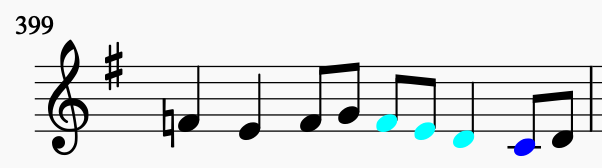
\includegraphics[width=0.35\textwidth]{paper/figs/cento_overlap_1.png}
    \caption{"FEDC" sequence due to FED (cyan) and EDC (blue) cento overlapping}
    \label{fig:cento_overlap_1}
\end{figure}

\begin{figure}[h]
    \centering
    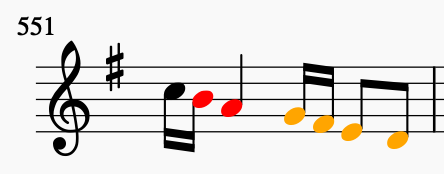
\includegraphics[width=0.3\textwidth]{paper/figs/cento_overlap_2.png}
    \caption{"BAGF\#ED" sequence due to cento overlapping}
    \label{fig:cento_overlap_2}
\end{figure}

\subsection{Analysis for the excluded centos}

The appendix also includes plots for the two theoretical centos, ‘AGB’ and ‘CDE’, which were not considered because they were not regarded as significant by the computational approaches. The plots show that although not substantial in frequency, these centos may convey crucial structural information about the form. For example, in Bassit, it appears that the cento 'AGB' is important for the conclusion of the mīzān. This points to the limitation of using repetition as the sole metric for the importance of a cento in AAM.

\subsection{General thoughts}

From a high-level visual analysis of the plots and by only observing repetition, we see patterns emerging both vertically (amongst centos) and horizontally (across time and musical structure).

Given the human nature of music, we might deduce that such ordered structures observed in the plots can be attributed to deliberate melodic developments.

Horizontally, we can see that these patterns coincide with the piece's structural sections, indicating intentional organization and developmental processes. The plots clearly reveal that a strong structure and repeating elements help make each section feel familiar and connected.

Vertically, the observed patterns reveal an apparent interdependence and correlation between repeated centos within sections of the piece in what appears to be kind of a "call and response" phenomenon between centos.

Also, it is important to note that several sections are devoid of centos altogether and there are instances where their repetition seems somewhat random. Also, while there are observable vertical and horizontal patterns within a score, we were unable to observe any singular pattern relating centos across the board.

\section{Conclusion and future work}\label{sec:Conclusion}

The study reveals a deliberate and purposeful scheme of motif repetition in Arab-Andalusian music with variations across rhythmic modes and the musical structure of a nawba in \textit{ṭab‘ ‘irāqal-‘ajam}. It points to a possibility that motif repetition might be a tool used in this tradition for creating cohesion, guiding listeners through structural boundaries, enhancing the overall musical narrative, and partially validating \cite{Chaachoo2011} theory.

By utilizing systematic musicology and computational techniques to analyze motif repetition quantitatively and qualitatively, we were able to get a glimpse into implicit structural patterns that may exist in Arab-Andalusian music. These observations contribute to the centonization theory of Arab-Andalusian music and may serve as a template for similar analysis at a larger scale. 

In the future, we could expand the scope to analyze other \textit{ṭubū‘} and eventually, the entire corpus. Alternately, finer statistical analysis techniques could be applied to the data generated from this study to identify concrete patterns of repetition and the role and interrelationship between the centos in a \textit{ṭab‘} in Arab-Andalusian music.\\

Generally speaking, a computation and data-driven approach to the study of Arab-Andalusian music could greatly contribute to the musicological study of this tradition. 

% For bibtex users:
\bibliography{ISMIRtemplate}





\newpage

% Include the PDF file at the end of the document
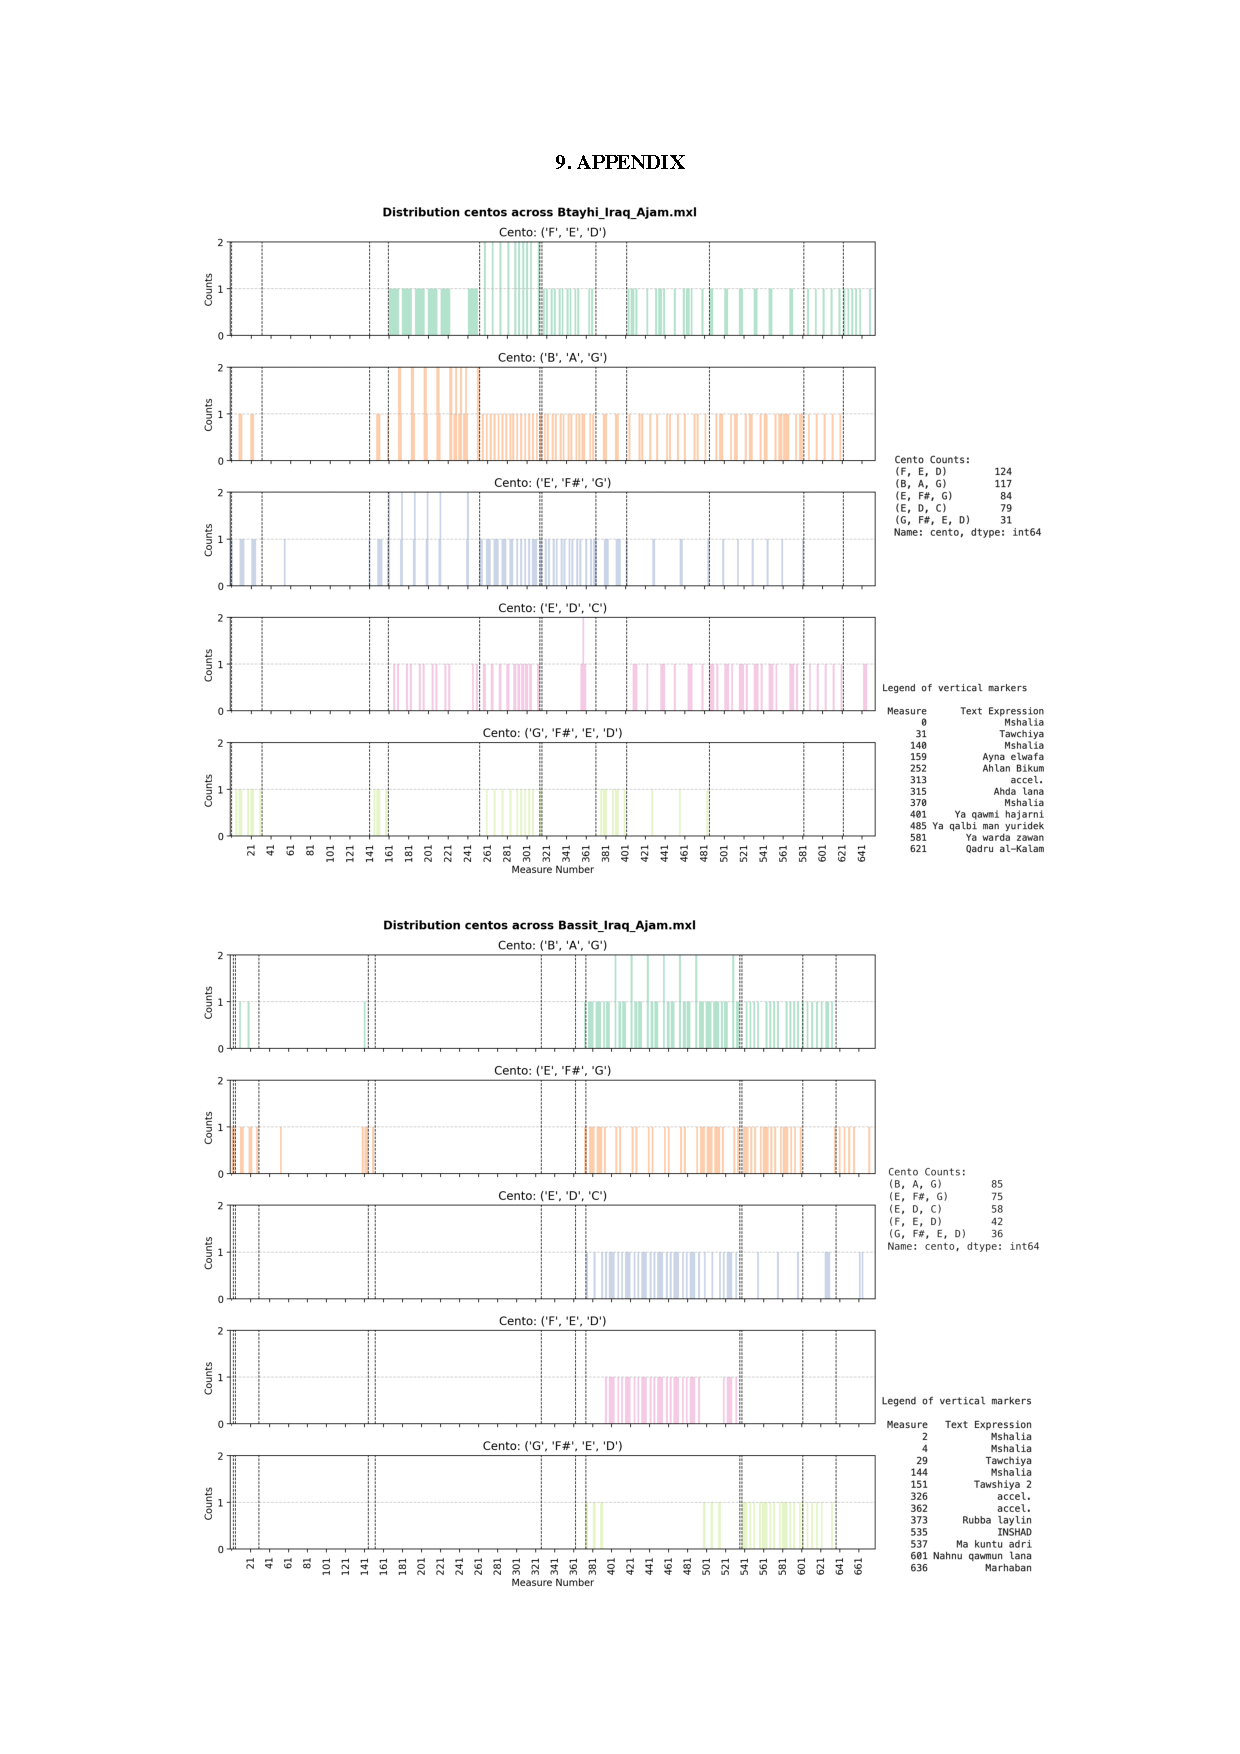
\includepdf[pages=-]{paper/figs/Appendix.pdf}

\end{document}

